\documentclass[12pt, letterpaper]{article}

% Packages
\usepackage[utf8]{inputenc}
\usepackage[sorting=none]{biblatex}
\usepackage{amsmath}
\usepackage{tabularx}
\usepackage{graphicx}
\usepackage{csquotes}
\usepackage{float}
\usepackage[normalem]{ulem}
\usepackage{subcaption}
\usepackage{authblk}
\usepackage{array}

% Bibliography
\addbibresource{./bib/Ma_2020.bib}
\addbibresource{./bib/rnn-effectiveness.bib}
\addbibresource{./bib/Understanding_LSTM.bib}
\addbibresource{./bib/Ramamoorthy.bib}
\addbibresource{./bib/Ramamoorthy2.bib}
\addbibresource{./bib/bahdanau2014neural.bib}
\addbibresource{./bib/a_tool_of_conversation.bib}
\addbibresource{./bib/racketracer.bib}
\addbibresource{./bib/Techlabs_2018.bib}
\addbibresource{./bib/tensorlayer2017.bib}
\addbibresource{./bib/nltk.bib}
\addbibresource{./bib/Kostadinov_2019.bib}
\addbibresource{./bib/Vinyals_Kaiser_Koo_Petrov_Sutskever_Hinton_2015.bib}
\addbibresource{./bib/google_s2s.bib}
\addbibresource{./bib/tf_softmax.bib}
\addbibresource{./bib/Khandelwal_2020.bib}
\addbibresource{./bib/tf_wb.bib}
\addbibresource{./bib/gfg_seq2seq.bib}
\addbibresource{./bib/Britz_2015.bib}
\addbibresource{./bib/tf_masking_padding.bib}

% Parragraph formatting
\setlength{\parskip}{1em}

\title{Implementación de un Chatbot utilizando una Red Neuronal Seq2Seq}

\author[1]{Nathaniel Calderón González}
\author[2]{Ernesto Mancebo Tavárez}
\affil[1]{MULCIA, Universidad de Sevilla, Sevilla, España}

\date{Junio 2020}

\begin{document}
    \begin{titlepage}
        \maketitle
        \begin{abstract}
            A continuación se presenta la memoria de un estudio de la implementación de un chatbot mediante el uso de una Red Neuronal bajo la arquitectura Seq2Seq, la misma es entrenada utilizando el Corpus de mensajes del microblog Twitter.
        \end{abstract}
    \end{titlepage}

    \tableofcontents
    \pagebreak

    \section{Objeto de Estudio}
    [PENDIENTE]
    
    \section{Marco Teórico}
    \subsection{Redes Recurrentes - RNN}
        A medida que se analizan estructuras tales como una fotografía, todo el contenido es capturado a la vez y el mismo no cambia a través del tiempo mas no toda la información es analizada de esta manera; existen estructuras donde se depende de la evolución de la misma para conocer su significancia, es decir, se necesita conocer en un determinado punto sus valores previos, es por ello que necesitamos herramientas que traten la información de manera secuencial [Cita Naranjo].
    
        Para solventar esto se tienen las Redes Neuronales Recurrentes (RNN) las cuales son diseñadas para el análisis de secuencias. Estas redes se caracterizan por lo siguiente:
        
        \begin{itemize}
            \item Comparten parámetros.
            \item Capaces de procesar secuencias de distintas longitudes.
            \item Detectan información relevante que pueden aparecer en distintas posiciones de la secuencia.
        \end{itemize}
        A modo de ejemplificar la última característica de estas redes se tiene \emph{`El 23 de Enero salí a pasear'} o \emph{`Salí a pasear el 23 de Enero'}. 
    
        Las RNN no conocen el significado de los símbolos que procesan, éstas infieren en el significado a partir de la extructura de la secuencia y la posición de los símbolos. Por otro lado, una RNN es capáz de lograr todo lo mencionado por el hecho de que tales redes tienen un estado al que en ocasiones se le puede escuchar referir como \emph{memoria}.
    
        El estado o memoria de tal red se logra a partir del hecho de que una RNN son redes con bucles dentro de ella.
    
        \begin{figure}[H]
            \centering
            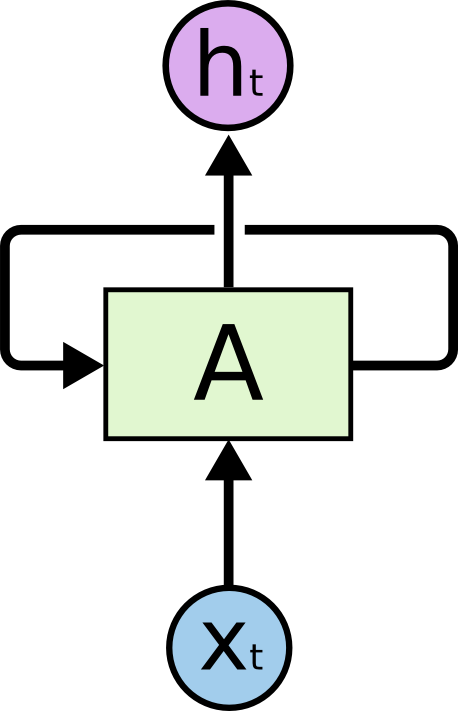
\includegraphics[width=0.2\linewidth]{img/RNN-rolled.png}
            \caption{Ilustración de una RNN.}
        \end{figure}
    
        En la representación se tiene un trozo de red $A$, la cual toma como entrada un $x_t$ y emite un valor $h_t$, de este modo, utilizando el bucle mencionado la información pasa al siguiente paso dentro de la red. Dicho ya esto, podemos ilustrar una red recurrente como una red con múltiples copias de sí misma\cite{Understanding_LSTM}.
    
        \begin{figure}[H]
            \centering
            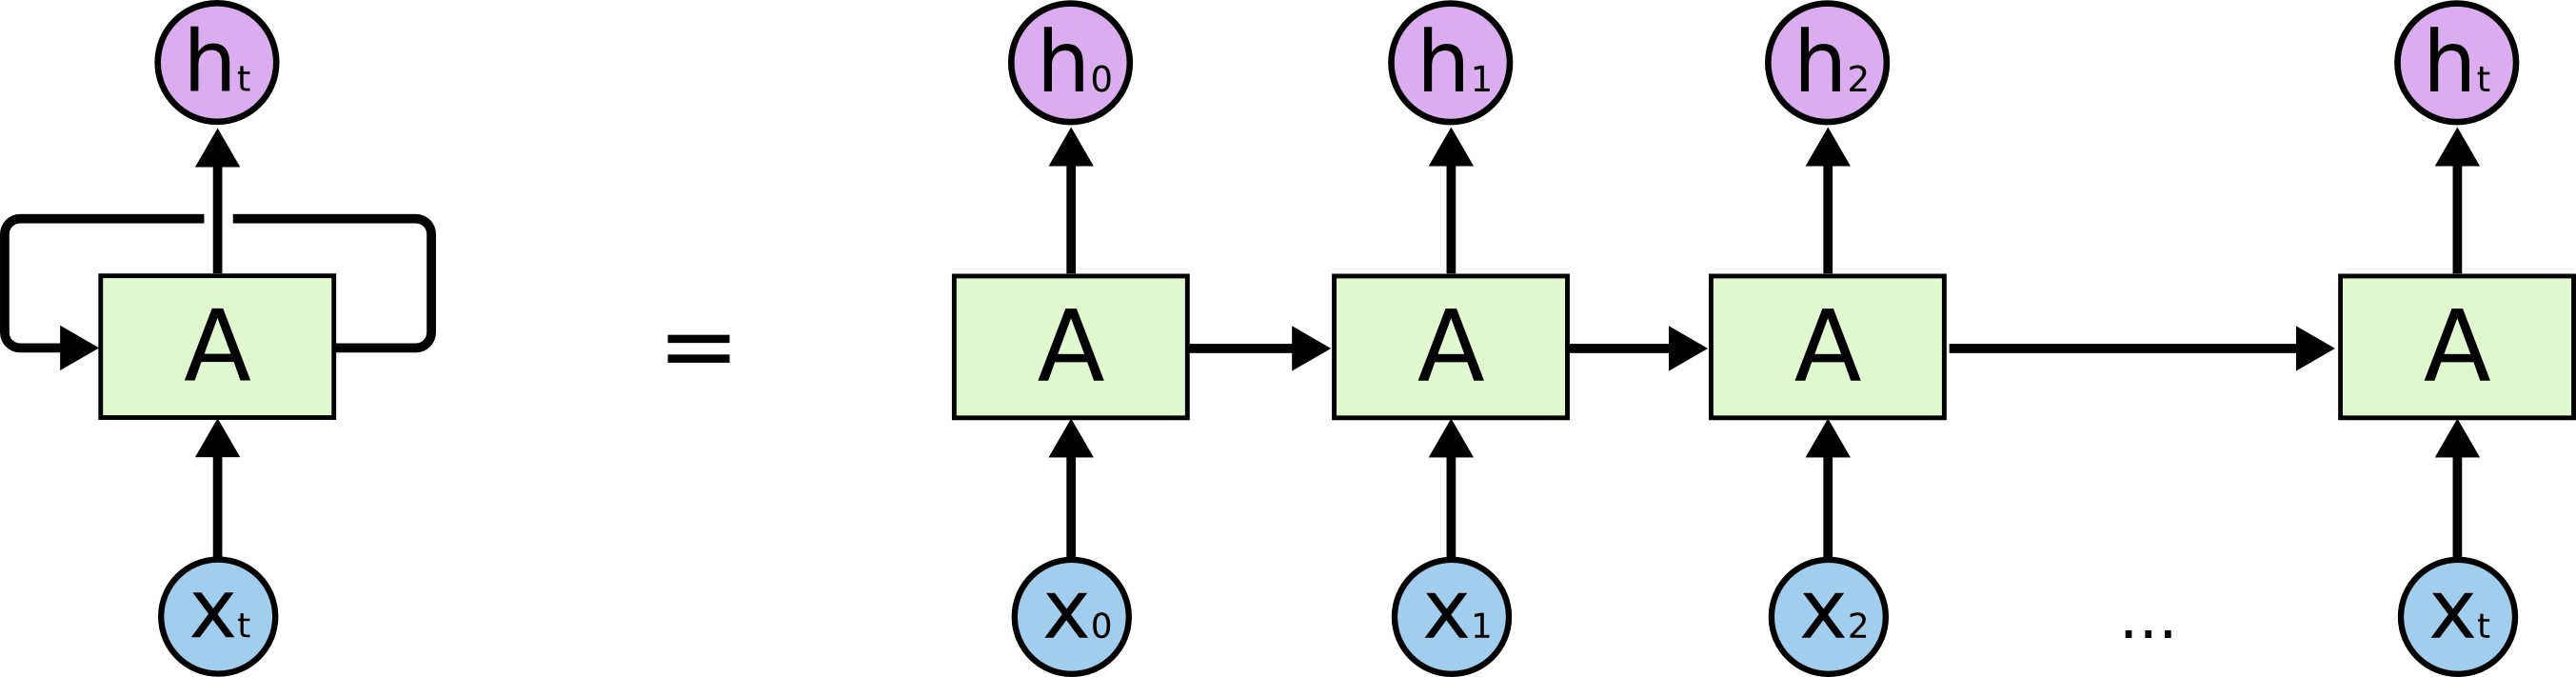
\includegraphics[width=\linewidth]{img/RNN-unrolled.png}
            \caption{Ilustración de la evolución de una RNN a través del tiempo $t$.}
        \end{figure}
        [REVISAR TEXTO]
        Este comportamiento en secuencia es lo que enlaza las RNN con secuencias y listas, por ellos, tales redes son exitosas para problemas de reconocimiento de voz, modelado del lenguaje, traducción, contextualización de imágenes y otras aplicaciones relacionadas\cite{rnn-effectiveness}.

    \subsection{Gated Recurrent Unit (GRU)}
    Las redes Gated Recurrent Unit, en lo adelante GRU, son un tipo de red recurrente(RNN) más sofisticadas que las RNN tradicionales y no sufren de desvanecimiento del gradiente, un problema típico en las RNN.
    
    Las redes GRU utilizan dos compuertas para mitigar los problemas del gradiente:
    \begin{itemize}
        \item Compuerta de actualización \emph{(Update Gate)}.
        \item Compuerta de reinicio \emph{(Reset Gate)}.
    \end{itemize}
    
    Estas compuertas representan dos vectores de la red que deciden qué información retener y qué información descartar con respecto al vector de información de salida de la red.
    
    El siguiente diagrama esboza el flujo de la red:

        \begin{figure}[H]
            \centering
            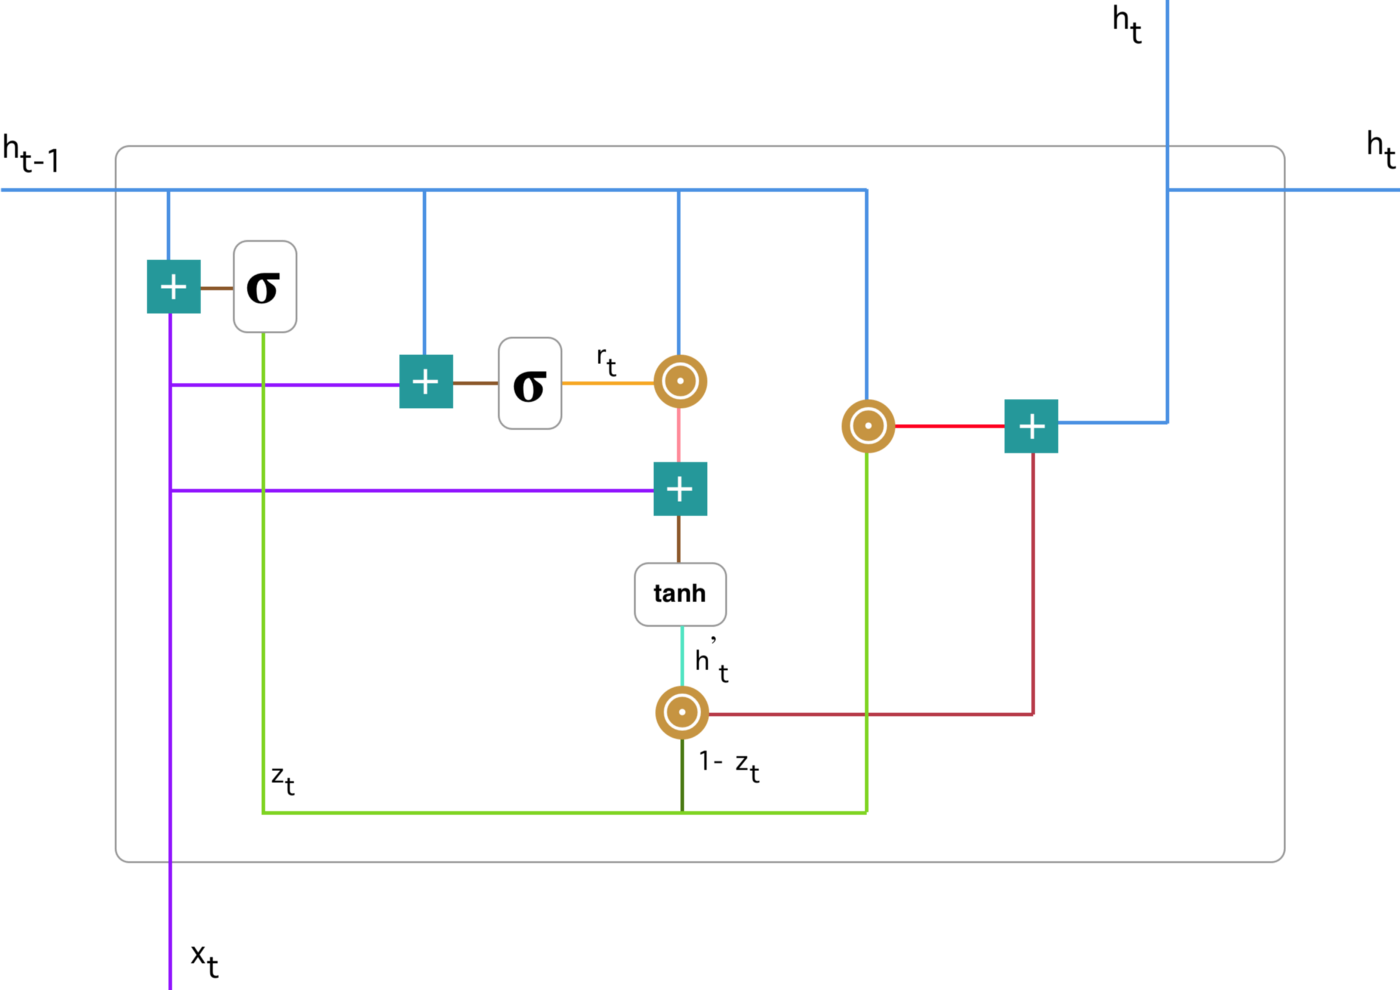
\includegraphics[width=0.8\linewidth]{img/gru_net.png}
            \caption{Ilustración de una red GRU.}
        \end{figure}

    La notación utilizada corresponde a la terminología común manejada en el área de aprendizaje automático, las cuales se definen como:
    
    \begin{itemize}
        \item $\sigma$: Función Sigmoide.
        \item $\text{tanh}$: Función Tangente Hiperbólica.
        \item $\odot$: Operación Producto Hadamard.
        \item $+$: Operación Adición. 
    \end{itemize}
    [LO DE ABAJO ES DE LA MISMA LISTA O NECESITA UNA ORIENTACION COMO LA LISTA DE ARRIBA??]
    \begin{itemize}
        \item $z_t$ representa la compuerta de actualización, la cual se calcula a partir de multiplicar el peso de la compuerta por $x_t$ y $h_{t-1}$, luego sumar los resultados y aplicar la función sigmoide.
        \begin{equation}
            z_t=\sigma(W^zx_t+U^zh_{t-q})
        \end{equation}
        \item $r_t$ representa la compuerta de reinicio, básicamente se calcula igual que la compuerta de actualización, solo que con sus pesos.
        \begin{equation}
            r_t=\sigma(W^rx_t+U^rh_{t-1})
        \end{equation}
        \item Entonces, la forma en que interviene la compuerta de reinicio para determinar qué información descartar de la celda estado o $h_t'$ es calculada de la siguiente forma:
        \begin{equation}
            h_t'=\text{tanh}(Wx_t + r_t\odot{Uh_{t-1}})
        \end{equation}
        Se multiplica $x_t$ por el peso $W$, y lo mismo para $h_{t-1}$ por el peso $U$ donde luego este resultado se usa para calcular el producto \emph{Hadamard} con $r_t$. Por último se suman ambos resultados y se aplica la tangente hiperbólica. Básicamente cuando $r_t$ tiende a $0$ pues significa que se debe descartar tal información.

        \item Finalmente, para calcular la celda estado $h_t$ se utiliza la fórmula:
        \begin{equation}
            h_t = z_t\odot{h_{t-1} + (1-z_t)\odot{h_t}}
        \end{equation}
        
        Donde se calcula el producto de Hadamard para la compuerta de actualización y la celda estado previa, y el producto de \emph{Hadamard} para la misma compuerta de actualización y la celda estado $h_t'$. En esencia si el vector $z_t$ tiende a uno pues retendrá la mayoría de la información previa y por consiguiente ignorando gran parte de la información actual\cite{Kostadinov_2019}.
    \end{itemize}

    \subsection{Redes Seq2Seq}
        Una implementación Seq2Seq consiste en dos redes recurrentes (RNN) enlazadas, una siendo codificadora y la otra decodificadora. La tarea de la codificador es leer una secuencia de entrada y emitir un contexto a partir del último estado oculto $h_t$ a partir de lo que considere importante en la secuencia de entrada. Posteriormente se tiene una red decodificadora la cual utiliza una función softmax sobre el vocabulario a utilizar para así emitir una secuencia de salida\cite{Ramamoorthy}\cite{Ramamoorthy2}.
    
        \begin{figure}[H]
            \centering
            \includegraphics[width=\linewidth]{img/Seq2Seq.png}
            \caption{Comportamiendo de una red Seq2Seq.}
        \end{figure}
    
        Se aprecia en la parte central de un modelo Seq2Seq lo que se conoce como \emph{Though Vector} o vector de pensamiento, el cuál representa la intención de la secuencia de entrada y a partir de aquí la sección decodificadora del modelo genera una secuencia a emitir, símbolo tras símbolo, palabra en este caso, donde cada símbolo es influenciado por el anterior.
    
    \subsection{Beam Search}
    Consiste en un algoritmo de búsqueda similar al Greedy Search, donde mientras Greedy Search siempre considera una única alternativa como la mejor, este algoritmo organiza las predicciones en forma de árbol y expande los nodos con mayor probabilidad.  Es necesario definir el Beam With o Top N lo cual limita a un número $n$ el número de alternativas que serán evaluadas en paralelo\cite{Khandelwal_2020}.
        
    \subsection{Contextualización de Palabra (Word Embedding)}
    La contextualización de palabras o word embedding, es una estrategia que permite vectorizar las palabras de un vocabulario de forma eficiente y en la que la codificación preserva la relación entre palabras. La contextualización de palabras es realizada usando una matriz de $n$ dimensiones de números reales los cuales representan pesos entrenables que son aprendidos durante el entrenamiento, de la misma forma que son aprendidos los pesos de una red. 
    
    \begin{figure}[H]
        \centering
        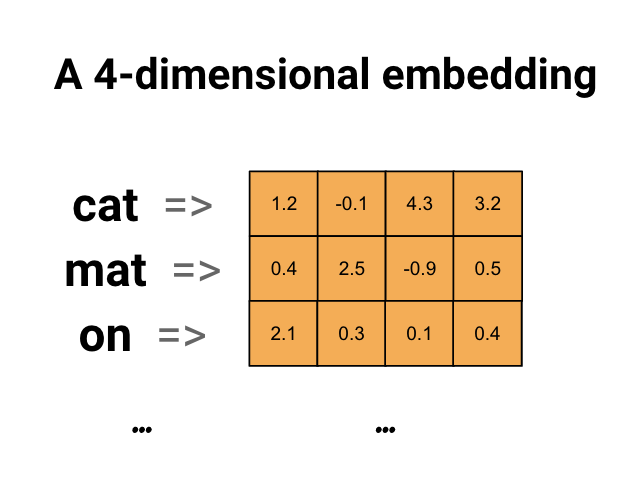
\includegraphics[width=0.8\linewidth]{img/4dim_embedding2.png}
        \caption{Ilustración de una matríz de Word Embedding.}
    \end{figure}
    A cada palabra del vocabulario del dataset se le asigna un índice en la matriz el cual es utilizado para referenciar la contextualización o \emph{"embedding"} a dicha palabra. Por esta razón se suele interpretar esta capa como una tabla de búsqueda, o \emph{"lookup table"}\cite{tf_wb}.

    \subsection{Tecnologías Utilizadas}
        \subsubsection{TensorLayer}
        Es una librería consistente en una extensión o una capa de alto nivel para la librería TensorFlow de Google. Esta librería al igual que TensorFlow permite realizar aprendizaje profundo \emph{(Deep Learning)} y aprendizaje por refuerzo \emph{(Reinforcement Learning)} pero aun nivel de abstracción superior, simplificando muchas de las tareas que comúnmente realizamos con TensorFlow.
        
        TensorLayer proporciona módulos de Aprendizaje Profundo y Aprendizaje por Refuerzo populares listos para ser usados, los cuales pueden ser modificados y adaptados a necesidades específicas de forma simple. Tal es el caso de la arquitectura de red Seq2Seq, la cual viene ya implementada y disponible para ser usada, y es la utilizada en este proyecto con ligeras modificaciones.
        
        También es importante destacar que a pesar de TensorLayer ser una librería de alto nivel, la misma no tiene efectos sobre el rendimiento de TensorFlow. Lo cual además de ser simple y flexible la hace aún más atractiva para la comunidad de científico de datos\cite{tensorlayer2017}.

        \subsubsection{NLTK}
        NLTK o Natural Language Toolkit, es una plataforma para trabajar con procesamiento del lenguaje natural en Python. NLTK cuenta con una coleccion de librerias para las típicas tareas de procesamiento de texto tales como, clasificación de textos, tokenización, análisis gramatical (parsing), razonamiento semántico, entre otros. NLTK también ofrece incorporado soporte a diferentes corpus y modelos de Aprendizaje Automático ya entrenados\cite{nltk}. 
        
        Para este proyecto se utilizó la última versión, NLTK 3, compatible con Python 3. Se utilizó NTLK para el preprocesamiento del corpus utilizando la función \emph{FreqDist} para obtener la distribución de frecuencia de las palabras del corpus.

    \section{Estado del Arte}
        \begin{table}[htb]
            \centering
            \resizebox{\textwidth}{!}{
                \begin{tabular}{|p{0.3\textwidth}|p{0.3\textwidth}|p{0.5\textwidth}|p{0.5\textwidth}|}
                    \hline
                    \textbf{Nombre} & \textbf{Plataforma} & \textbf{Propósito} & \textbf{Características} \\
                    \hline
                        @HotelReviewsBot\cite{racketracer} & Python, NLTK & Consultar cualidades de un Hotel registrado en http://www.hostelworld.com/ & Capturaba tweets que contenían enlaces a un hotel en el referido portal y extraía comentarios relevantes del hospedaje, ya sea sobre el wi-fi, desayuno, baño, ducha o ruido del lugar. \\
                        \hline
                        A Tool of Conversation: Chatbot\cite{a_tool_of_conversation} & Java, Java Applets, Base de Datos & Demostrar la implementación de un flujo conversacional a partir de un esquema de patrones & Sugiere el uso de patrones para encontrar preguntas ya registradas en la base de datos y de hallarla, dar una respuesta al usuario. \\
                        \hline
                        Chatbots Enlatados\cite{Techlabs_2018} & Computación en la Nube & Proveer a empresas soluciones listas para su uso & Tienden a estar asociadas a ciertas industrias de manera predefinidas, tales como restaurantes y tiendas en línea. \\
                        \hline
                        Practical Sec2Sec\cite{Ramamoorthy2} & Python, NLTK, Tensorflow & Chatbot capaz de dar respuestas coloquiales, a partir de lo aprendido de corpus como Twitter y Cornell Movies & Implementa una red neuronal utilizando Tensorflow la cual es entrenada a partir de un corpus de conversaciones. \\
                    \hline
                \end{tabular}
            }
            \caption{Estado del arte para implementaciones de Chatbots.}
        \end{table}

    \section{Corpus y Modelado de la Data}
        El corpus utilizado para entrenar esta red corresponde a un conjunto de más de 700 mil mensajes procedentes de la red social Twitter. Este corpus es provisto por el repositorio chat\_corpus\cite{Ma_2020} donde detalla que para las líneas impares corresponden a \emph{tweets} o mensajes emitidos y las líneas pares corresponden a respuestas al  \emph{tweet} predecesor.
        
        Para modelar este vasto conjunto de datos es preciso realizar una serie de pasos con la intención de reducir la complejidad de aprendizaje para la red a entrenar, pues el modelo Seq2Seq trae consigo varios retos y uno de ellos es la variabilidad de la longitud de la secuencias, por el hecho de que la longitud de las secuencias de entrada a procesar es indiscutiblemente variable. Otro problema destacable es la dimención del vocabulario a utilizar ya que sin duda alguna es ineficiente aplicar una función softmax para cada palabra del vocabulario con el cual trabajaremos\cite{Ramamoorthy}.
        
        \subsection{Conversión a minúscula}
        La primera tarea de preprocesado del corpus, todas las palabras en el mismo son llevadas a minúsculas con el objetivo de que palabras lexicográficamente equivalentes sean en un posterior paso consideradas al momento de evaluar su distribución.
        
        \subsection{Filtrado de caracteres}
        Cada carácter dentro para cada palabra es filtrado mediante una expresión regular de forma $[\text{a-z0-9}\backslash{s}]$, permitiéndonos tan solo procesar texto alfanumérico, evitando que la red considere escenarios complejos donde haya presencia de símbolos.
        
        \subsection{Ternas (Bucketing)}
        Es preciso para la entrenar una red Seq2Seq el que las secuencias de entrada sean de una misma longitud, siendo esto un inconveniente pues las secuencias en el corpus son variables en cuanto a longitud se trata. Para solventar esta situación existe lo conocido como ternas o “bucketing”, donde se elige un subconjunto tanto de preguntas como de respuestas las cuales entren dentro del rango establecido.
        
        Para el problema a tratar se tuvo el siguiente criterio, una terna o bucket $((0,20),(3,20))$ siendo el primer binomio el rango para las preguntas y el segundo el de respuestas, leído de forma: Una pregunta o secuencia de entrada debe de corresponder a una longitud no mayor a 20 palabras, mientras que una respuesta debe de constar entre tres y veinte palabras.
        
        \subsection{Indexado de Palabras}
        Este paso es uno de los más importantes y críticos de la implementación, pues se trata de crear una tabla de búsqueda en donde se tenga una distribución de frecuencia para cada palabra obtenida del paso anterior, siendo la primera en la lista la  palabra más utilizada y lo opuesto para la última palabra, dígase la menos frecuente. Asimismo, en la implementación estudiada la tabla obtenida es delimitada a tan solo las primeras seis mil palabras, por lo que se restringe el dominio del vocabulario a tal cantidad.
        
        La implementación de ésta técnica es lograda apoyándose en la ya expuesta librería NLTK y su función \emph{FreqDist}, y se ha de destacar que una vez obtenida la distribución de frecuencia para cada palabra en el corpus y restringido el dominio del vocabulario, se añaden en la cabecera de la lista los caracteres ‘\_’ que representan rellenado o “padding” y el caracter “unk” o desconocido para palabras fueras del vocabulario obtenido; estos caracteres sirven de apoyo a la red pues como se explicará en el apartado siguiente, es preciso tener tales caracteres para situaciones excepcionales a la cual nos enfrentaremos.
        
        [VER SI VALE LA PENA ESTA SUBSECCION]
        \subsection{Contextualización de Palabras (Word Embedding)}
        La contextualización de palabras es una técnica para el aprendizaje de representaciones densas de palabras dentro de un vector de reducida dimención. Se puede valorizar cada palabra como un punto en un espacio y tal espacio es representado por el vector ya referido. Relaciones semanticas entre palabras son obtenidas mediante ésta técnica pues tienen propiedades aproximadas.
    
        \begin{figure}[H]
            \centering
            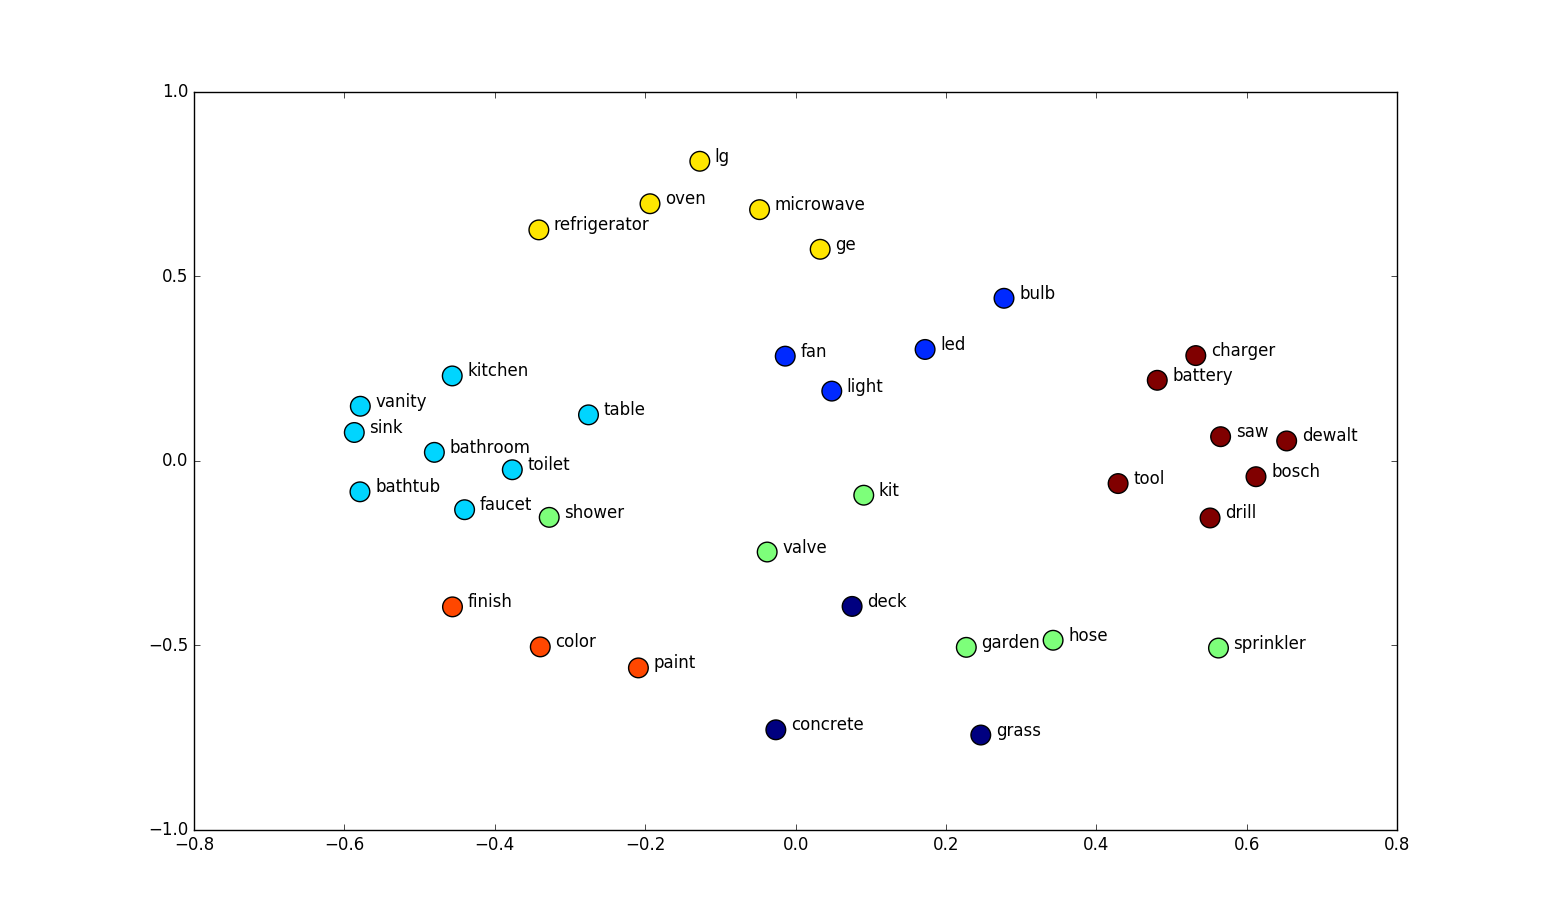
\includegraphics[width=\linewidth]{img/we1.png}
            \caption{Word Embedding.}
        \end{figure}
    
        Ésta tarea es típicamente aplicada en la primera fase de la red y esto se conoce como \emph{Embeding Layer}, donde se asocia una palabra (index to word in vocabulary) del vocabulario para un vector del tamaño dado. Para la arquitectura Seq2Seq los pesos de la capa \emph{Embeding Layer} son entrenados en conjunto con otros parámetros del modelo\cite{Ramamoorthy}.
        
        \subsection{Rellenado de Oraciones (Padding)}
        Como bien fue mencionado en el apartado “ternas”, es necesario al momento de entrenar que las secuencias utilizadas en la red  ocupen la misma dimensión, considerando el hecho de que existen secuencias de longitudes inferiores a veinte, siendo veinte el límite superior tanto para pregunta como respuesta. Es por esto que cada vector de secuencia el cual no alcance la dimensión mencionada para cada conjunto es acotado a tal dimensión, dígase veinte unidades, donde para las secuencias con menos de veinte unidades son rellenadas hasta alcanzar la dimensión en cuestión.


    \section{Arquitectura}
        \begin{figure}[H]
            \centering
            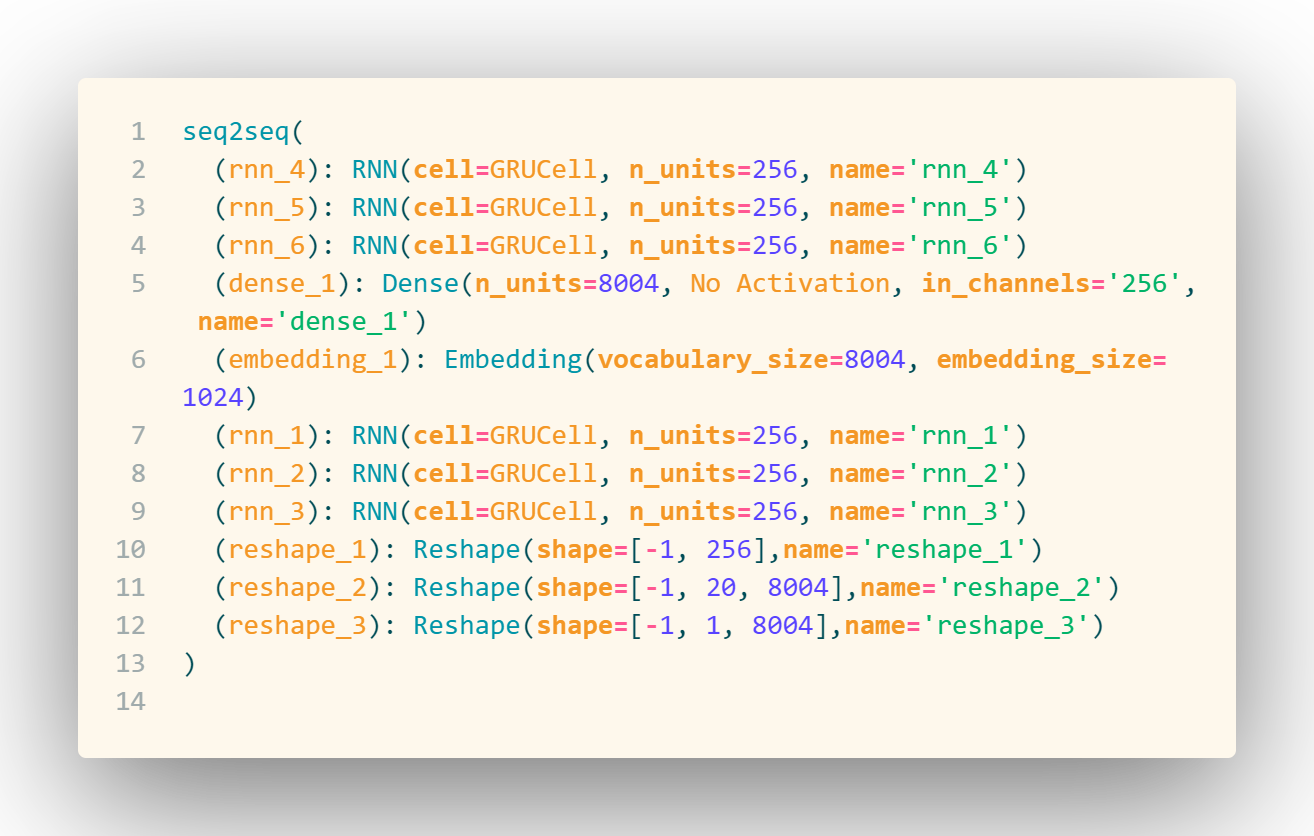
\includegraphics[width=0.8\linewidth]{img/code/seq2seq_arq.png}
            \caption{Arquitectura modelo Seq2Seq.}
        \end{figure}
        
        \begin{itemize}
            \item Embedding Layer(vocabulary\_size=8004, embedding\_size=1024)
            \item Codificador:
                \begin{itemize}
                    \item 3 - GRU Layer de 256 unidades
                    \item Embedding Layer(vocabulary\_size=8004, embedding\_size=1024)
                \end{itemize}
            \item Decodificador
                \begin{itemize}
                    \item 3 - GRU Layer de 256 unidades
                \end{itemize}
            \item Reshape Layer (shape(-1,256))
            \item Dense Layer de 8004 unidades, recibe una entrada de un tensor de 256 canales(shape=(1, 256)).
            \item Reshape Layer (shape(-1, 1, 8004))
            \item Capa de contextualización de palabras o Word Embedding, se utiliza previo a pasar el vector de ID de las palabras de la secuencia de entrada al codificador. También se usa previo a pasar el token especial "start\_id" al decodificador.
            \item Codificador
                \begin{itemize}
                    \item Esta conformado por tres capas GRU(GRUCell), de 256 unidades cada una.
                    \item Convierte las palabras de la secuencia de entrada en vectores de estados ocultos. Cada vector de estado oculto representa una palabra y el contexto de esta.
                \end{itemize}
            \item Decodificador
            \begin{itemize}
                \item Tambien esta conformado por tres capas GRU(GRUCell), de 256 unidades cada una.
                \item La capa inicial recibe de entrada un vector con el token especial "start\_id" y se le pasan los estados ocultos del codificador como los estados iniciales del stack capas.
                \item El codificador predice palabra por palabra la secuencia de salida, recibiendo en cada paso en el tiempo, o instante T:
                \begin{enumerate}
                    \item Un contexto de todas las palabras hasta ese instante.
                    \item Los estados ocultos producidos hasta ese instante.
                \end{enumerate}
                \item Para maximizar la probabilidad de la palabra producida se utiliza el algoritmo de búsqueda Beam Search con número de 3 alternativas definido por defecto, también conocido como "top n" o "beam width".
                \item La computación termina cuando se produce el número de palabras definido como threshold. Para este caso fue una secuencia de máximo 20 palabras.
            \end{itemize}
        \end{itemize}

        La salida del codificador es un vector de 20 palabras con él se produce la salida final concatenando palabra por palabra hasta encontrar el token especial \emph{"end\_id"}\cite{tensorlayer2017}\cite{gfg_seq2seq}.

    \section{Entrenamiento y Creación del modelo}
        \begin{figure}[H]
            \centering
            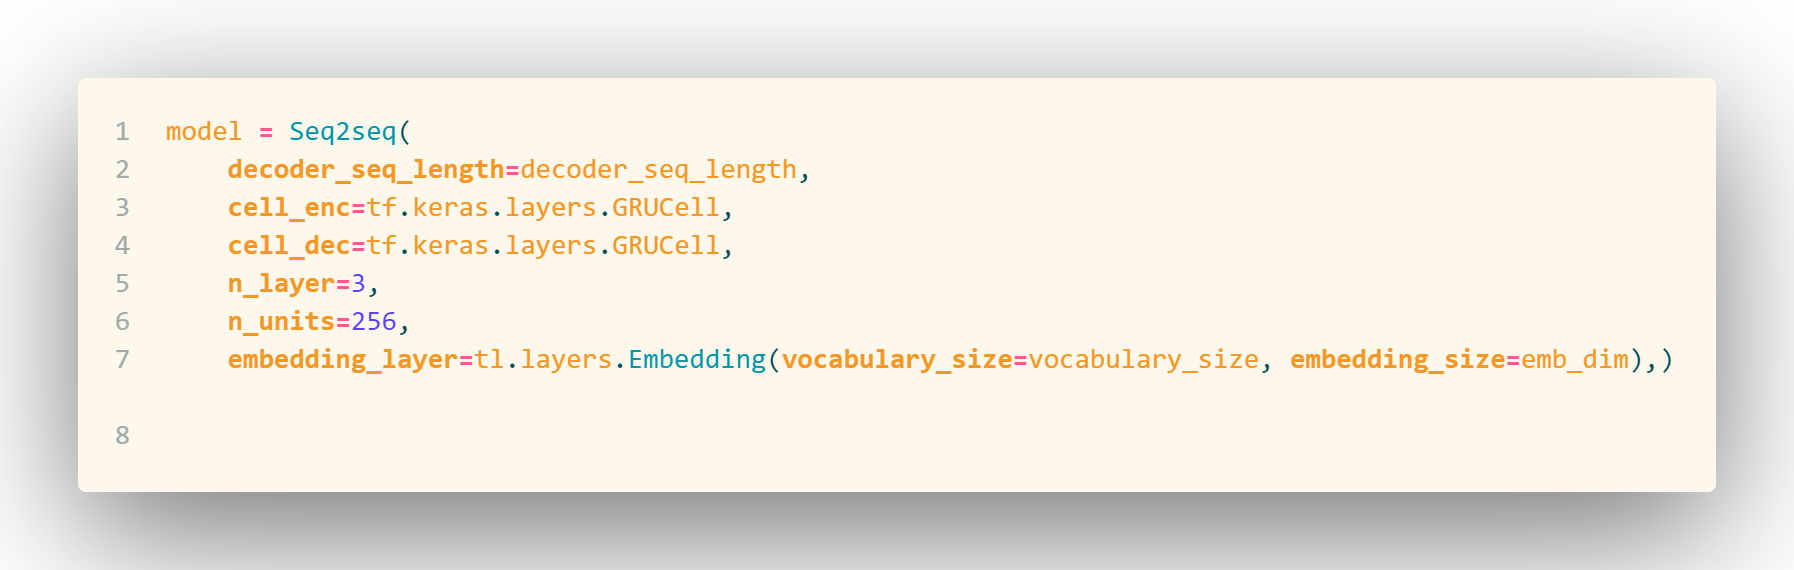
\includegraphics[width=0.8\linewidth]{img/code/seq2seq_model.png}
            \caption{Creación del modeloSeq2Seq.}
        \end{figure}

        Para llevar a cabo el entrenamiento de la red neuronal ya descrita, es utilizado el corpus preprocesado resultante de apartados anteriores, donde tal corpus es segmentado en las siguientes proporciones: un 70\% del conjunto de datos es utilizado para entrenamiento, un 15\% para prueba y el 15\% restante para validación\cite{Britz_2015}.

        Asimismo, el entrenamiento de la red es realizado durante una serie de 50 epochs y en cada epoch le es suministrado como ejemplo un subconjunto o batch de 32 instancias. 
        
        [VER SI SAMPLING VA]
        Se utilizan dos tokens especiales como prefijo y sufijo de cada secuencia, “start\_id” y “end\_id" respectivamente. Donde a la hora de realizar sampling, “start\_id" es el token que representa el inicio de la secuencia, y “end\_id", representa el final, lo cual permite saber cuando terminar la operación de sampling.
        
        Posteriormente se evalúa las predicciones del modelo a partir de la salida del mismo y se calcula la pérdida mediante el cálculo de entropía cruzada utilizando la función cross\_entropy\_seq\_with\_mask provista por tensorflow, el valor computado como pérdida es utilizado para calcular el ajuste del gradiente para los pesos de la red y posteriormente es aplicado a tales pesos, esto ocurre durante cada iteración o epoch.

    \section{Diálogo con el Modelo (Inference)}
        Tras el oportuno entrenamiento del modelo el mismo es evaluado proveyendo al mismo un texto o secuencia de entrada, respondiendo el modelo una secuencia de salida. Se ha de destacar que todo esto es apoyado en la tabla de indexado que se construye en la fase de modelado del corpus, donde la entrada digitada es llevada a su representación numérica, y la salida de la red es llevada a texto por el proceso inverso, buscando la equivalencia de cada índice con una palabra, y la unión de este vector es la secuencia producto legible por el usuario.
        
        A continuación se muestra una tabla donde se ilustran las preguntas y respuestas obtenidas por quienes elaboraron este proyecto. Es importante resaltar que el dominio de las preguntas y respuestas se circunscribe al contenido observado en el corpus.

    [tabla]

    \section{Conclusiones}

    \pagebreak
    \printbibliography[title={Bibliografía}]
\end{document}